
	\documentclass{article}
	\usepackage{amsmath,amssymb}
	\usepackage[inline]{enumitem}
	\usepackage{blindtext}
	\usepackage{booktabs}
	\usepackage{graphicx}
	\usepackage{xcolor}
	\usepackage[vmargin = 1.5in, top = 1in, bottom = 1.2in, letterpaper]{geometry}
	\usepackage{listings}
	\usepackage{courier}
	\usepackage{multicol}
	\usepackage{multirow}
	\usepackage{bm}
	\usepackage{subcaption}
	\lstset{
	basicstyle = \small\tt,
	keywordstyle = \tt\color{blue},
	commentstyle = \it\color[cmyk]{1,0,1,0},
	stringstyle = \tt\color[RGB]{128,0,0},
	%frame = single,
	backgroundcolor = \color[RGB]{245,245,244},
	breaklines,
	extendedchars = false,
	xleftmargin = 2em,
	xrightmargin = 2em,
	aboveskip = 1em,
	tabsize = 4,
	showspaces = false
	}
	\begin{document}
	
	% \newfontfamily\courier{Courier New}

	
	\title{STAT 520 Homework 3}
	\author{Yifan Zhu}
	\maketitle
	
	\begin{enumerate}[leftmargin = 0 em, label = 3.\arabic*., font = \bfseries]
	\item 
	\begin{enumerate}[label = \arabic*.]
		\item Random variable in this question is OXY and the covariate is body mass.

		 \item 
		 By doing Box-Cox plot with 6 bins in Figure \ref{Box-Cox}, we find a straight line could be used to roughly describe the relation between log mean and log standard deviation, with a slope of about 1.09. That suggests a variance function of something like $V(\mu_i) = \mu_i^{2.18}$. While for gamma random component we have $\mu_i^2$, I would choose the random component of this model to be \textbf{gamma}.
		 \begin{figure}[!htb]
		 	\centering
		 	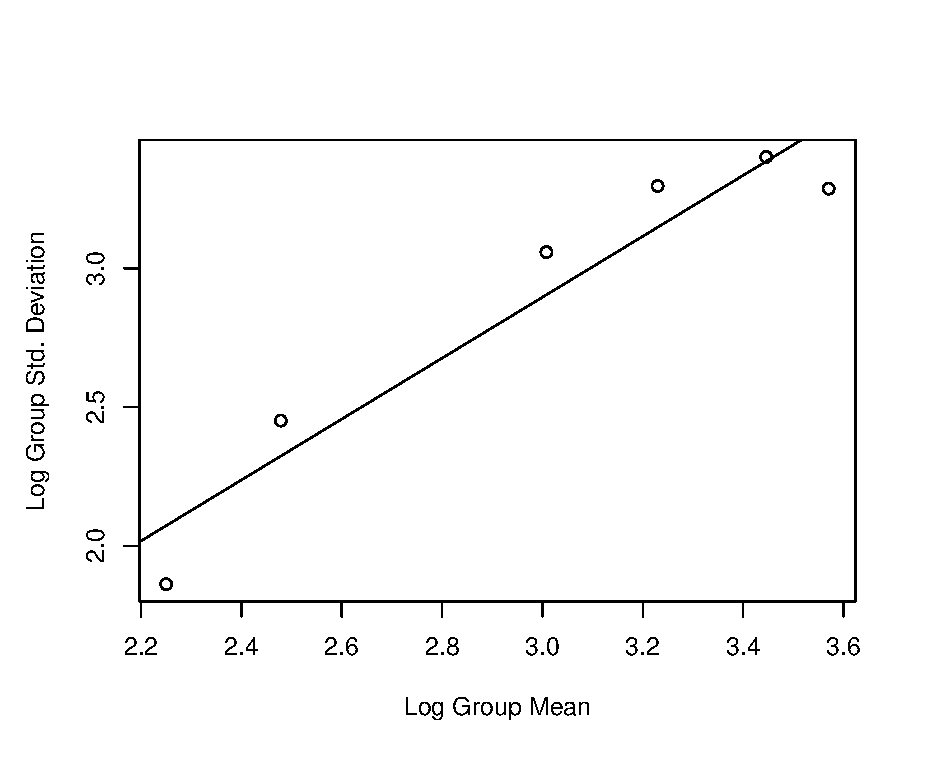
\includegraphics[width = 0.8\textwidth]{Box-Cox.eps}
		 	\caption{Box-Cox Plot from OXY and body mass}
		 	\label{Box-Cox}
		 \end{figure}

		 \newpage
		 \item 
		 In the plot of the logarithm of responses against the covariate values in Figure \ref{link}. With the exception of a couple of points, a straight line seems to be a reasonable description of this plot, so we might try a model with \textbf{gamma random component} and \textbf{log link}. 
		 \begin{figure}[!htb]
		 	\centering
		 	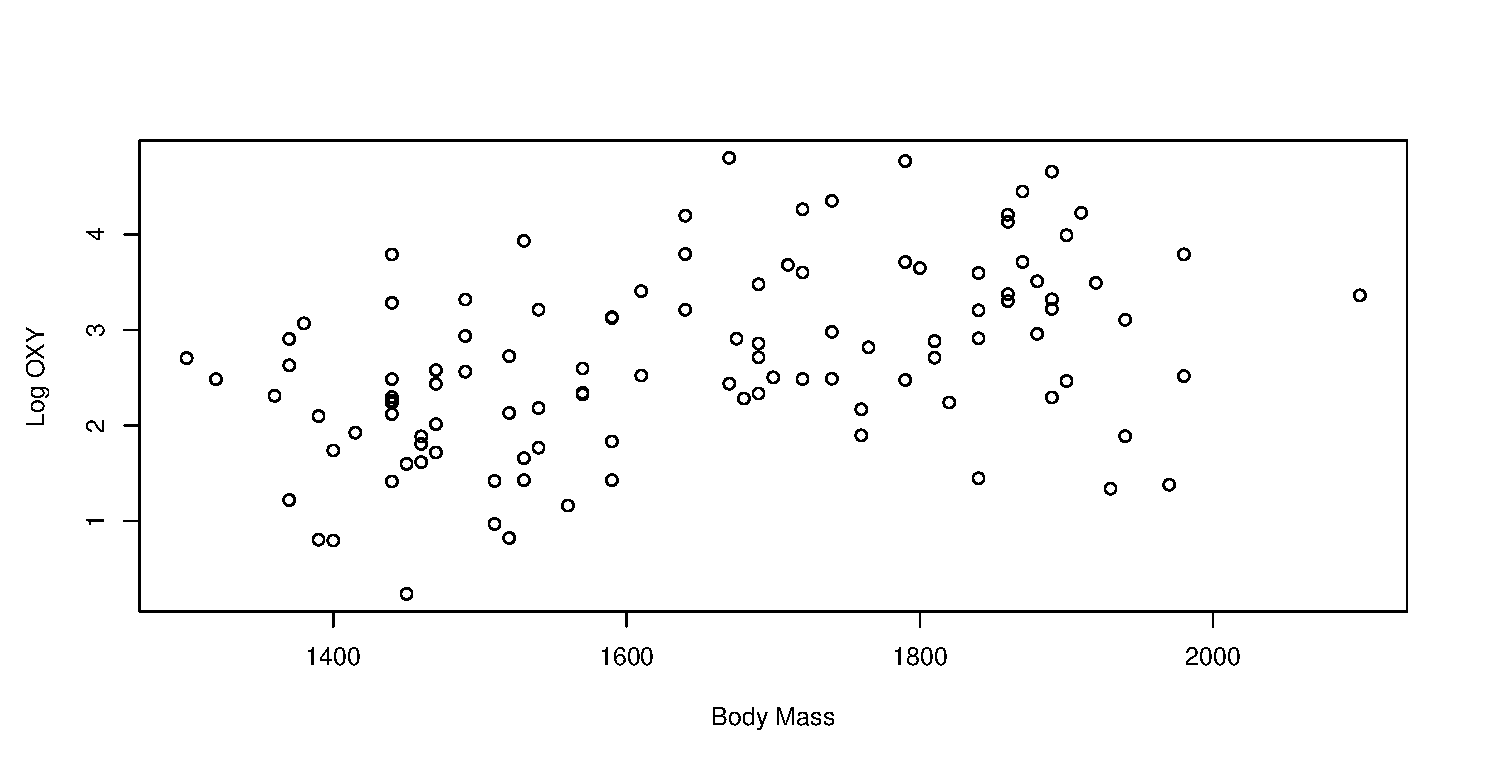
\includegraphics[width = 0.8\textwidth]{Find_Link.eps}
		 	\caption{Scatterplot of log transformed responses against covariates}
		 	\label{link}
		 \end{figure}

		 And after fitting this model, we gave the residual plots in Figure \ref{res} and from the one with log fitted values we can see the residual plot is pretty good. Hence the log link function not a bad choice here. 

		 \begin{figure}[!htb]
		 \centering
		 	\begin{subfigure}{0.5\textwidth}
		 	\centering
		 	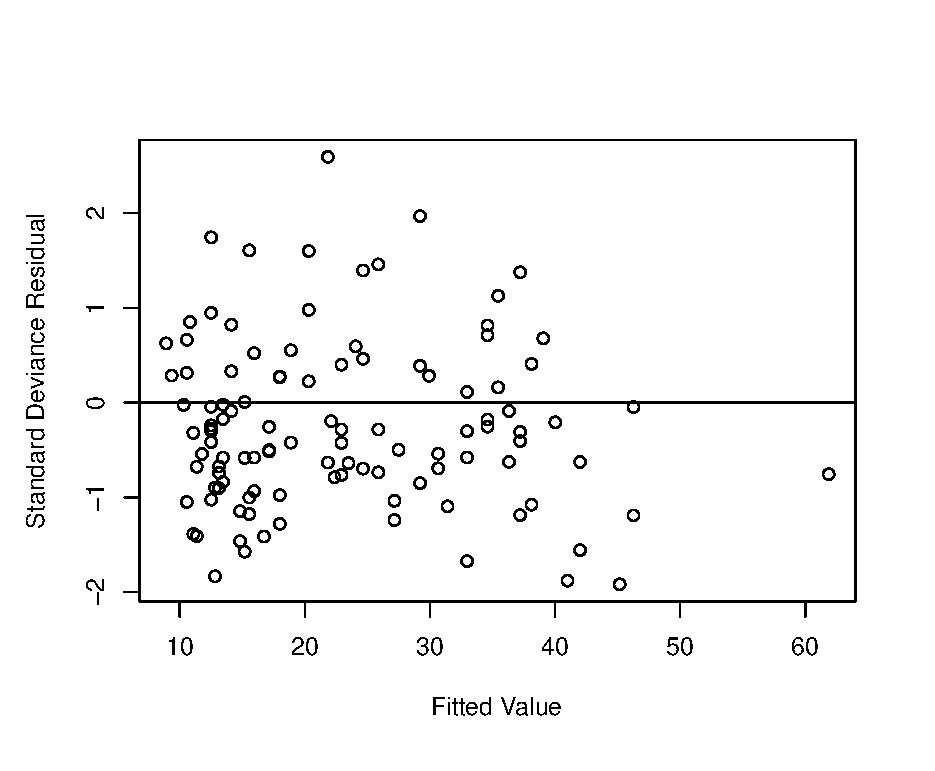
\includegraphics[width = \linewidth]{resplot1.eps}
		 	\caption{}
		 	\end{subfigure}%
		 	~
		 	\begin{subfigure}{0.5\textwidth}
		 	\centering
		 		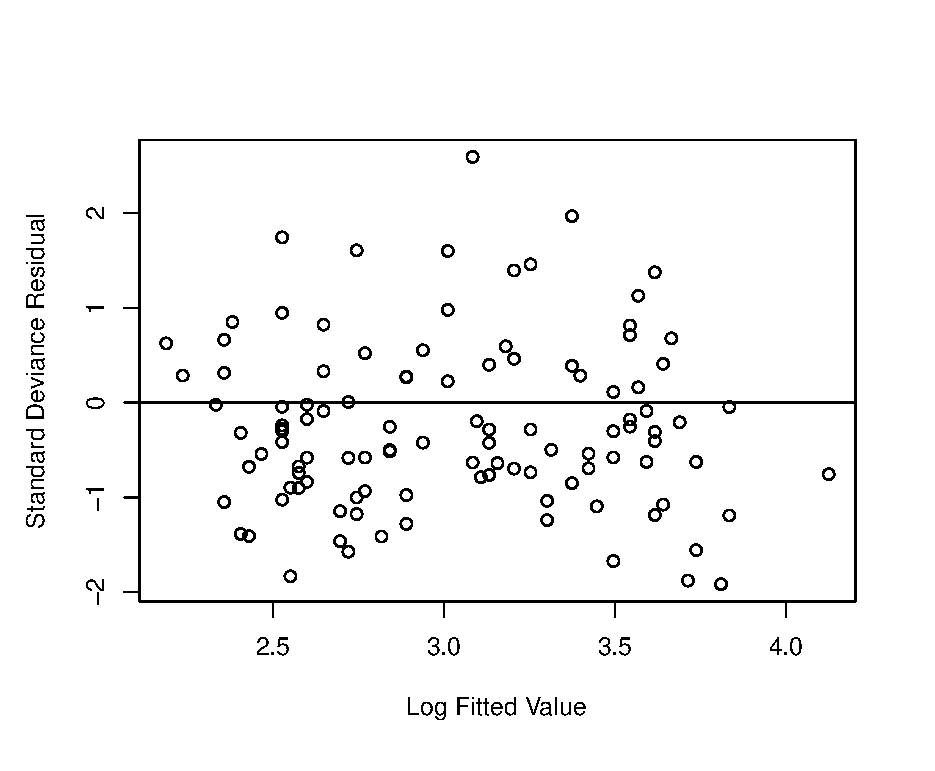
\includegraphics[width = \linewidth]{resplot2.eps}
		 		\caption{}
		 	\end{subfigure}
		 	\caption{Residual Plots}
		 	\label{res}
		 \end{figure}

		 \newpage
		 \item Results of fitting a basic GLM:



		 \begin{center}
		 \begin{tabular}{ll}
		 \toprule
		 $\hat{\beta}_0$ & -0.9605936\\
		 $\hat{\beta}_1$ & 0.002421781\\ 
		 95 \% CI for $\hat{\beta}_0$ &(-2.47653, 0.5553304)\\
		 95 \% CI for $\hat{\beta}_1$ &(0.001487, 0.0033130)\\
		 unscaled deviance & 76.5991\\
		 scaled deviance & 89.41392\\
		 log likelihood for fitted model &  -144.0595\\
		 log likelihood for saturated model &  -99.35258\\
		 \bottomrule
		 \end{tabular}
		 \end{center}
		 \begin{figure}[!htb]
		 	\centering
		 	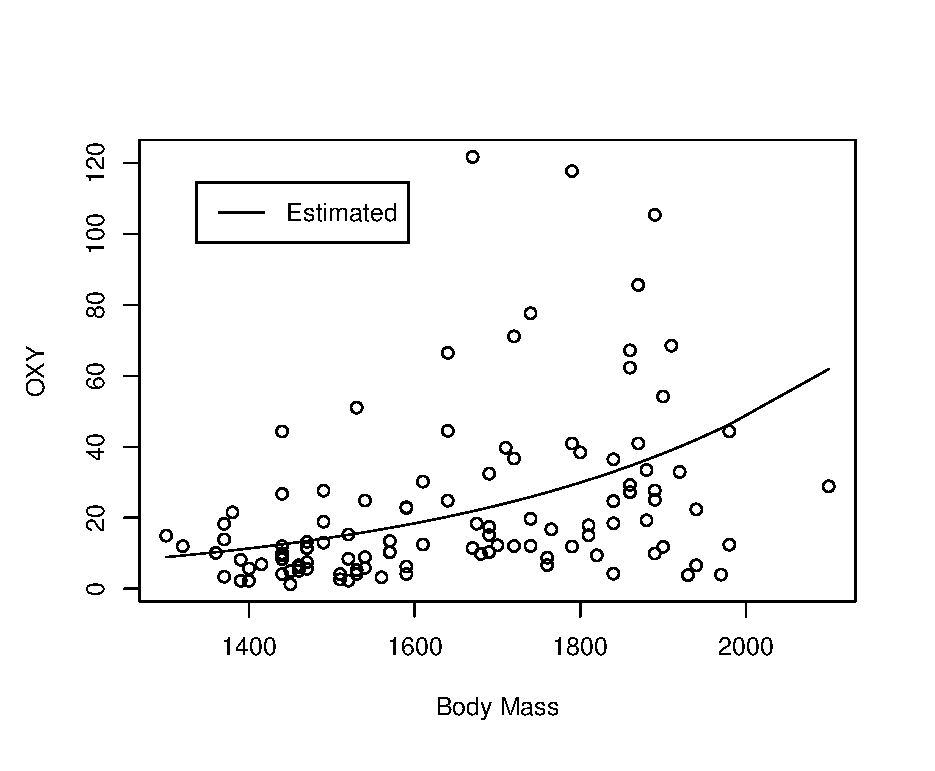
\includegraphics[width =  0.8\textwidth]{estimates.eps}
		 	\caption{Scatter plot and estimated expected value}
		 	\label{estimated}
		 \end{figure}
		 




	\end{enumerate}
	
	\newpage
	\item 
	\begin{enumerate}[label = \arabic*.]
		\item 
		Scatter plot of simulated data:
		\begin{figure}[!htb]
			\centering
			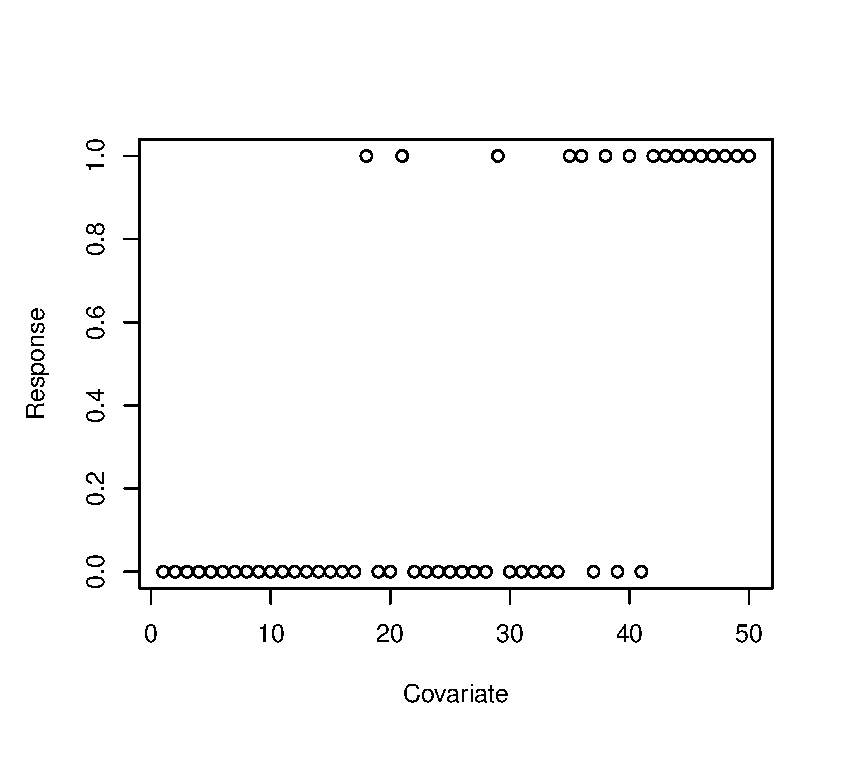
\includegraphics[width = 0.8\textwidth]{2scatter.eps}
			\caption{Scatter plot of simulated data}
			\label{2scatter}
		\end{figure}

		\begin{center}
		 \begin{tabular}{ll}
		 \toprule
		 $\hat{\beta}_0$ & -5.253796\\
		 $\hat{\beta}_1$ & 0.1365626\\ 
		 95 \% CI for $\hat{\beta}_0$ &(-7.81967727, -2.6879138)\\
		 95 \% CI for $\hat{\beta}_1$ &(0.06938077, 0.2037445)\\
		 unscaled deviance & 33.63338\\
		 scaled deviance & 33.63338\\
		 log likelihood for fitted model &  -16.82295\\
		 \bottomrule
		 \end{tabular}
		 \end{center}

		 \newpage
		 The fitted line and true line are shown in Figure \ref{2true}:
		 \vspace{-1.2em}
		 	\begin{figure}[!htb]
			\centering
			\includegraphics[width = 0.8\textwidth]{2truees.eps}
			\caption{True and estimated line}
			\label{2true}
		\end{figure}


\newpage
		\item Fitted expectations and pointwise 95\% confidence band:
				 \vspace{-1.2em}
			\begin{figure}[!htb]
			\centering
			\includegraphics[width = 0.8\textwidth]{2ci.eps}
			\caption{Fitted line with 95\% pointwise confidence band}
			\label{2ci}
		\end{figure}



	\end{enumerate}
	



 	\end{enumerate}


	
	
	
	\end{document}